\subsection{Mobkom The Player}

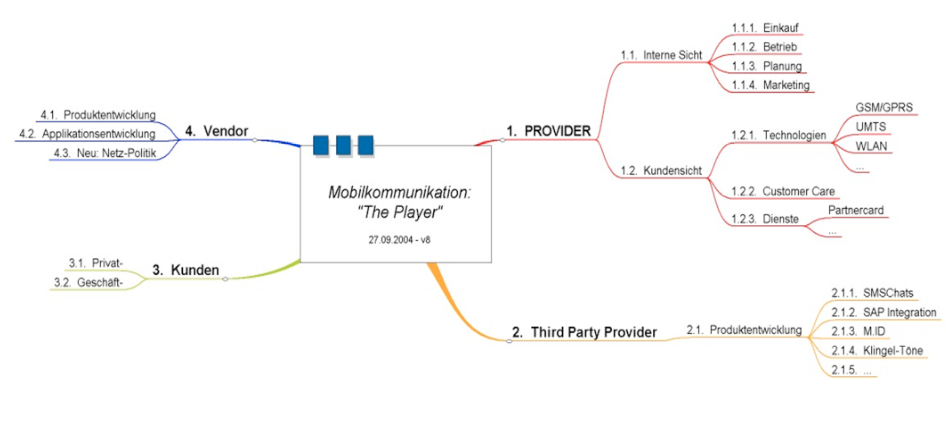
\includegraphics[height = 5 cm]{./Pics/MobKomThePlayer}

\subsection{Mokom Generell}
\begin{minipage}{0.5 \linewidth}
\begin{itemize}
\item sicherheitskritisches 
\item simultan laufendes
\item Echtzeit
\item Zeit abweichendes
\item non-stop
\item Fehlertolerantes
\item  uneinheitliches
\item dezentrales System
\end{itemize}
\end{minipage}
\begin{minipage}{0.5 \linewidth}
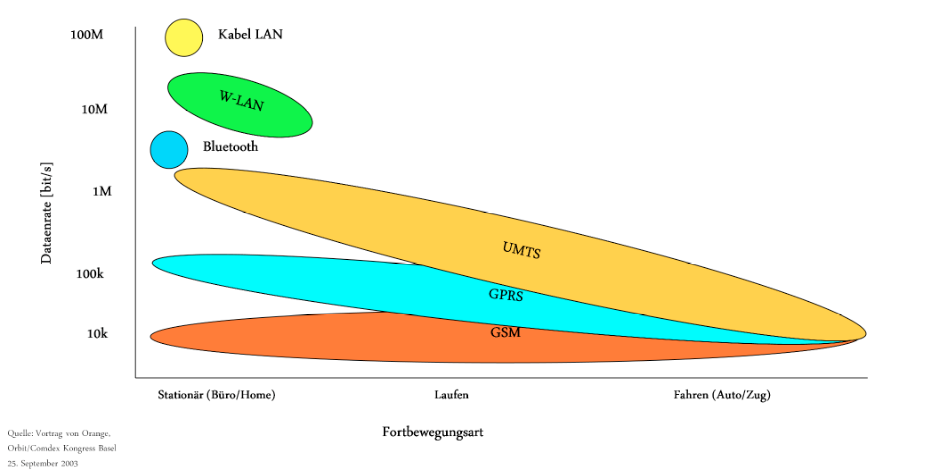
\includegraphics[width = \linewidth]{./Pics/Technologien}
\end{minipage}

\subsection{Multiplexing}
\subsubsection{Raum-Multiplex}
Raum wird in verschiedene Bereiche aufgeteilt und jedem Konkurrenten/Teilnehmer ein Bereich zugewisen, so dsas diese sich bei zeitgleicher Nutzung nicht gegenseiteig beeinflussen können. \\
\textbf{Beispiel :} Mobilfunk-Zellenaufteilung, Kabelbündel

\subsubsection{Zeit-Multiplex TDMA}
Das Medium der Kommunikation darf von jedem Konkurrenten exklusiv für eine bestimmte Periode genutzt werden (Zeitabschnitt wird zugewiesen, fest oder zufällig je nach Bedarf) \\
\textbf{Beispiel :} Festnetzte,GSM,IEEE 802,3 (CSMA/CD)

\subsubsection{Frequenz-Muliplex FDMA}
Jedem Konkurrenten um das MEdium wird eine exklusive Frequenz zugewiesen, auf der er dann zeitgleich mit den anderen senden kann.
\textbf{Beispiel :} Radio-/TV-Frequenz, GSM-Netz, Betriebsfunknetze,Glasfasernetze

\subsubsection{Code-Multiplex CDMA}
Zuordnung exklusiver Codes zu einzelnen Sendern, so dass alle gleichzeitig auf einer identischen Frequenz senden können, aber anhand des Codes eindeutig identifiziert werden können.
\textbf{Beispiel :} UMTS

\subsection{Störung}
\subsubsection{Abschattung}
Durch Hindernisse kann ein Signal abgeschattet (shadowing) werden. Der Empfang wird dadurch erschwert oder verhindert
\textbf{Beispiel :} Hochhäuser, Tunnel

\subsubsection{Reflexion}
Wellenförmiges Signal wird an grosser Fläche (spiegelartig) reflektiert. Reflektierte Signale sind schwächer als direkt empfangene (wenn sie denn überhaupt empfangen werden)

\subsubsection{Streuung}
Relativ kleine Hindernisse können das Signal streuen (scattering), das sich dann in verschiedene Richtungen weiterbewegt.

\subsubsection{Beugung}
Kanten können eine Beugung (diffraction)/Ablenkung des Signals verursachen.

\subsubsection{Dämpfung \& Verzögerung}
Empfangsleistung nimmt proportional zum Quadrat der Entfernung zwischen Sender und Empfänger ab(path loss). Zeitrahmensynchronisation ist ortsabhängig (time alginment)

\subsubsection{Interferenzen}
Konkurrieren mehrer Mobilstationen um das Übertragungsmedium können Interferenzen (Überlagerung zwischen getrennten Kanälen) auftreten.

\subsubsection{Mehrwegausbreitung-Multipath Fading}
\begin{itemize}
\item Aufgrund von Streuung, Beugung und REflexion kann das Signal das Ziel auf unterschiedlichen Wegen erreichen.
\item Der Impuls des Senders kann beim Empfänger mehrfach und zeitlich versetzt auftreten.
\item Die Stärke der eingehenden Signale schwankt, da die Ausbreitungswege unterschiedliche Dämpfung aufweisen können.
\item Unterschieden wird zwischen 
\begin{itemize}
\item Rayleigh Fading 
\item Time Dispersion
\end{itemize}
\end{itemize}

\subsection{Zellplanung}
Die Zentrale frage ist, wie viele Zellen werden für die Netzabdeckung der Region benötigt. Die Zellplanung ist abhängig von:
\begin{itemize}
\item Anzahl Kanäle pro Zelle
\item die mittlere Anzahl der Teilnehmer pro Zelle (steuerbar über die grösse der Zelle)
\item Qualität des angebotenen Dienstes (Grade Of Service GOS)
\item der mittlere Verkehr, den die Teilnehmer pro Zelle produzieren, ist abhängig von der
\begin{itemize}
\item Populationsverteilung
\item Verteilung Autobenutzung
\item Verteilung des Einkommens in der Region
\item Charakteristik der landestypischen Telefonierverhaltens 
\item Telefonstatistik
\item Anzahl der Kunden (subscriber) des Mobilfunkanbieters
\end{itemize}
\end{itemize}
\begin{multicols}{2}
\begin{eqnarray}
A = \frac{n \cdot T}{3600 s} \\
\left[ A \right] = \frac{\left[ s \right] }{\left[ s \right] } = \text{Pseudoeinheit Erlang} \\
B = \frac{\frac{A^n}{n!}}{\sum_{i = 0}^{n} \frac{A^i}{i!}}
\end{eqnarray}
\columnbreak

In 1 und 2:
\begin{itemize}
\item A = Angebotener Verkehr
\item n = mittlere Anzahl der Anrufe pro Zelle
\item T = mittlere Dauer eines Gespräches
\end{itemize}
In 3:
\begin{itemize}
\item A = Angebotener Verkehr zur Hauptverkehrsstunde
\item n  = Anzahl Kanäle
\item B = Blockierwahrscheinlichkeit
\end{itemize}
\end{multicols}
\subsubsection{Verlustsysteme}

Reine Wartesysteme existieren in der Praxis nicht. Jedoch kann mit Annäherungen gearbeitet werden, wenn die Anzahl zur Verfügung stehenden Warteplätze gegenüber der mittleren Warteschlangenlänge ausreichend gross ist. \\

Die Verlustwahrscheinlichkeit lässt sich mit der Erlang B Funktion berechnen. Die Formel ist oben und die Verlustwahrscheinlichkeit ist gleich der Blockierwahrscheinlichkeit.


\newpage